\documentclass[14pt,russian,a4paper]{extarticle}

\usepackage[a4paper,left=30mm,right=15mm,top=20mm,bottom=20mm,bindingoffset=0cm]{geometry}
\usepackage{amsfonts,amssymb,amsmath,enumerate,float}
\usepackage{cmap}
\usepackage{ifthen}
\usepackage[utf8]{inputenc}
\usepackage[T2A]{fontenc}
\usepackage[russian]{babel}

\usepackage{graphicx}
\usepackage[font=small,labelfont=bf]{caption}
\usepackage{hyperref}


\linespread{1.5}

\begin{document}

\thispagestyle{empty}

{\footnotesize 

\begin{center}
    МИНИСТЕРСТВО ОБРАЗОВАНИЯ И НАУКИ РОССИЙСКОЙ ФЕДЕРАЦИИ \\
    ФЕДЕРАЛЬНОЕ ГОСУДАРСТВЕННОЕ АВТОНОМНОЕ ОБРАЗОВАТЕЛЬНОЕ \\
    УЧРЕЖДЕНИЕ ВЫСШЕГО ОБРАЗОВАНИЯ \\
    \guillemotleft НОВОСИБИРСКИЙ НАЦИОНАЛЬНЫЙ ИССЛЕДОВАТЕЛЬСКИЙ ГОСУДАРСТВЕННЫЙ \\
    УНИВЕРСИТЕТ\guillemotright (НОВОСИБИРСКИЙ ГОСУДАРСТВЕННЫЙ УНИВЕРСИТЕТ, НГУ)
\end{center}

\vspace{4mm}

\begin{flushleft}
    Факультет {\bf ФИЗИЧЕСКИЙ} \\
    Кафедра {\bf ФИЗИКО-ТЕХНИЧЕСКОЙ ИНФОРМАТИКИ}
\end{flushleft}
\begin{flushleft}
    Направление подготовки {\bf 03.04.02 ФИЗИКА} \\
    Образовательная программа {\bf МАГИСТРАТУРА}
\end{flushleft}

\vspace{4mm}


\begin{center}
    {\bf
    ВЫПУСКНАЯ КВАЛИФИКАЦИОННАЯ РАБОТА \\
    МАГИСТЕРСКАЯ ДИССЕРТАЦИЯ
    }
\end{center}

\begin{center}
    {\bf Герасёв Алексей Владимирович}
\end{center}

\begin{center}
    Тема работы: {\bf Разработка системы управления быстрыми компонентами электронно-лучевой установки}
\end{center}

\vspace{4mm}

\leftline{\bf \guillemotleft К защите допущена\guillemotright}

\vspace{2mm}

\noindent
\begin{minipage}[t]{70mm}
    \begin{center}
    {\bf Заведующий кафедрой} \\
    учёная степень, звание \\
    должность, место работы \\
    Логашенко И. Б. / \makebox[20mm]{\dotfill} \\
    \guillemotleft\makebox[10mm]{\dotfill}\guillemotright \makebox[30mm]{\dotfill} 20\makebox[5mm]{\dotfill} г.
    \end{center}
\end{minipage}
\hfill
\begin{minipage}[t]{70mm}
    \begin{center}
    {\bf Научный руководитель} \\
    учёная степень, звание \\
    должность, место работы \\
    Болховитянов Д. Ю. / \makebox[20mm]{\dotfill} \\
    \guillemotleft\makebox[10mm]{\dotfill}\guillemotright \makebox[30mm]{\dotfill} 20\makebox[5mm]{\dotfill} г. \\
    учёная степень, звание \\
    должность, место работы \\
    Чеблаков П. Б. / \makebox[20mm]{\dotfill} \\
    \guillemotleft\makebox[10mm]{\dotfill}\guillemotright \makebox[30mm]{\dotfill} 20\makebox[5mm]{\dotfill} г.
    \end{center}
\end{minipage}

\vspace{4mm}

\begin{flushright}
    Дата защиты: \guillemotleft\makebox[10mm]{\dotfill}\guillemotright \makebox[30mm]{\dotfill} 20\makebox[5mm]{\dotfill} г.
\end{flushright}

\vfill

\centerline{Новосибирск, 2018}
}

\newpage
\thispagestyle{empty}
\tableofcontents
\newpage

\section{Введение}

\subsection{Электронно-лучевые технологии}
В последнее время электронно-лучевые технологии всё шире используются в науке и промышленности. Принцип работы основан на том, что мощный пучок электронов попадает на материал объекта, помещённого в вакуум, и локально нагревает его до высоких температур. Данный подход используется для точной резки и сварки металлов, в том числе химически активных, тугоплавких и разнородных. Так как есть возможность получить достаточно узкий пучок высокой мощности, данная технология позволяет добиться высокой точности обработки материала. Также с недавнего времени широкое развитие получают такие направления электронно-лучевых технологий как аддитивные (к которым относится трёхмерная печать) и ионно-плазменные.

\subsection{Электронно-лучевые установки в ИЯФ}
В настоящее время в Институте Ядерной Физики СО РАН ведутся работы по развитию электронно-лучевых технологий \cite{weld_coord}. В ИЯФ СО РАН были разработаны, собраны и запущены несколько электронно-лучевых установок. Одна из этих установок (так называемая "малая" установка) является экспериментальной и используется для разработки и изучения новых электронно-лучевых технологий. При разработке малой установки был применён ряд уникальных технических решений (например, альфа-магнит \cite{alpha_magnet} и лазерный подогрев катода \cite{laser_heat}), а также проведён ряд уникальных экспериментов (3D-печать вольфрамом \cite{wolfram_3d} и т.д.).

\section{Основная часть}
Устройство и механизм сцепления DMA-блоков изображён на рис. \ref{fig:dma}.
\begin{figure}[h!]
    \centerline{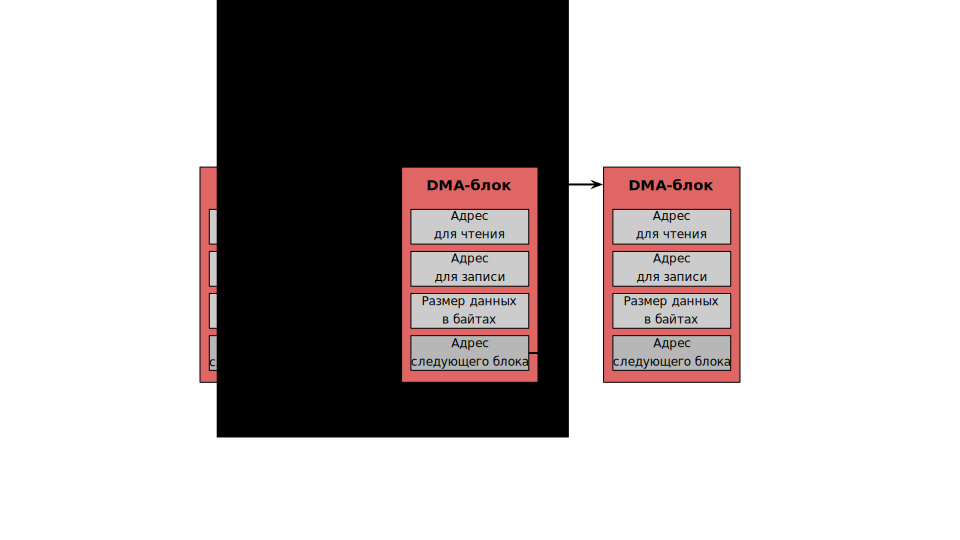
\includegraphics[width=400pt]{media/dma_chain.pdf}}
    \caption{Устройство DMA-блоков}
    \label{fig:dma}
\end{figure}

\section{Заключение}
\section{Литература}

\begin{thebibliography}{99}

\bibitem{weld_coord}
Купер Э.А., Логачев П.В., Репков В.В., Селиванов А.Н., Селиванов П.А., Семенов Ю.И., Трибендис А.Г., Федотов М.Г., Чертовских А.С. -
Автоматизированная система для задания координат шва в установках электронно-лучевой сварки. –
Автометрия. Издательство СО РАН. Новосибирск. – 2015. – Том 51, №1. – С. 55 – 61.

\bibitem{wolfram_3d}
Семенов Юрий Игнатьевич, Алякринский О.Н., Болховитянов Д.Ю., Логачев П.В., Медведев А.М., Спесивцев А.Б., Старостенко А.А., Яминов К.Р. -
Макет 3D принтера для изготовления металлических структур из тугоплавких металлов с помощью электронно-лучевых аддитивных технологий. -
Институт ядерной физики им. Г.И. Будкера СО РАН (Новосибирск), Россия. -
\url{http://conf.ict.nsc.ru/clapt2015/ru/program}

\bibitem{alpha_magnet}
О.Н. Алякринский, М.А. Батазова, Д.Ю. Болховитянов, М.Ю. Косачев, П.В. Логачев, А.М. Медведев, Ю.И. Семенов, М.М. Сизов, А.А. Старостенко, А.С. Цыганов. Прототип источника электронов с магнитным поворотом пучка для электронно-лучевых технологий.

\bibitem{laser_heat}
О.Н. Алякринский, К.В. Губин, М.Ю. Косачев, Э.А. Купер, П.В. Логачев, А.М. Медведев, В.К. Овчар, В.В. Репков, Ю.И. Семенов, М.М. Сизов, А.А. Старостенко, М.Г. Федотов, А.С. Цыганов. Прототип источника пучка электронов с лазерным подогревом катода.

\end{thebibliography}

\section{Приложения}

\end{document}
